\documentclass[tikz,border=10pt]{standalone}
\usetikzlibrary{calc}
\begin{document}
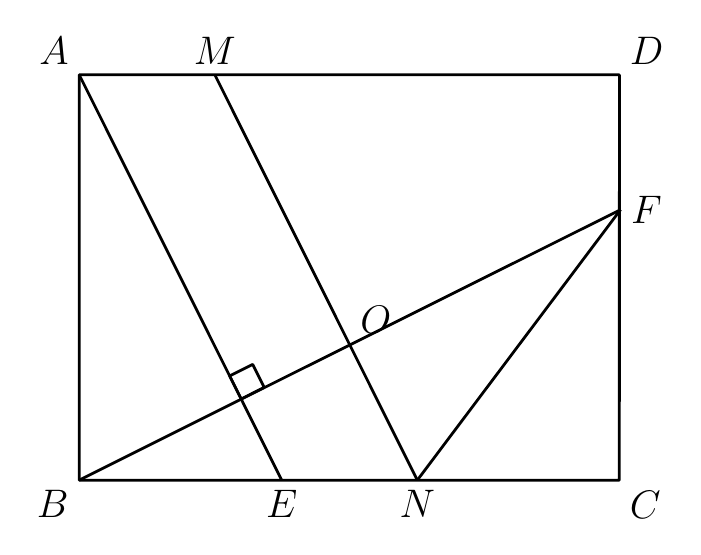
\begin{tikzpicture}[line join=round, line width=1.0pt,
  lbl/.style={font=\fontsize{14.5}{17.4}\selectfont}]
% Scale s = 0.018141 cm/px, origin at rectangle centre (257,207) px, y flipped
\coordinate (A) at (-3.4316059591763675,2.5749208964911863);
\coordinate (D) at (3.428914997830909,2.5743479467441452);
\coordinate (B) at (-3.432035945823966,-2.5737547462142256);
\coordinate (C) at (3.42848501118331,-2.5743276959612666);
\coordinate (M) at (-1.7092240897558955,2.574777053441573);
\coordinate (E) at (-0.8595081369187575,-2.5739695883765923);
\coordinate (N) at (0.8627738649670055,-2.573913514068957);
\coordinate (F) at (3.4439067563809886,0.8610818078523604);
\coordinate (O) at (0.003450319849959478,-0.8509252733332513);
\coordinate (P) at (-1.3744568185371853,-1.5429368865749717);
% Right-angle square corners at P
\coordinate (Q1) at (-1.08177085393709,-1.3961098395727518);
\coordinate (Q2) at (-1.2280736033207065,-1.1033608022635144);
\coordinate (Q3) at (-1.5208598322284428,-1.2498880441129518);

% Rectangle
\draw (A) -- (D) -- (C) -- (B) -- cycle;
% Interior segments
\draw (A) -- (E);
\draw (M) -- (N);
\draw (B) -- (F);
\draw (N) -- (F);
% Right-angle marker at P
\draw (P) -- (Q1) -- (Q2) -- (Q3) -- cycle;

% Labels
\node[above left, lbl] at (A) {$A$};
\node[above right, lbl] at (D) {$D$};
\node[below left, lbl] at (B) {$B$};
\node[below right, lbl] at (C) {$C$};
\node[above, lbl] at (M) {$M$};
\node[below, lbl] at (E) {$E$};
\node[below, lbl] at (N) {$N$};
\node[right, lbl] at (F) {$F$};
\node[above right, lbl] at (O) {$O$};
\end{tikzpicture}
\end{document}